\section{Experiments}
\label{sec:experiments}

To demonstrate that our \emph{Intra-Process Pipe (IPP)} system is a practical solution to 
providing speedups without sacrificing the reliability and safety benefits of hardware isolation, 
we conducted experiments on both microbenchmarks and real-world workloads. 

\todo[inline]{Yiwen: Besides the performance results we are showing here, should we also add experiments 
demonstrating the reliability and safety of our system? Maybe we can show examples such as an attacker 
tried to access memory address in cage B from inside of Cage A, but failed. Or maybe we can talk about this 
in the Discussion section.}

\subsection{Microbenchmarks}
\label{experiments.microbenchmarks}

The purpose of our microbenchmark experiments was to demonstrate that by introducing intra-process pipe, 
communication between two processes through our user-space pipe would be faster than using the traditional 
pipe, which will invoke system calls into the operating system kernel that incur context switches. 

Our microbenchmark experiments were conducted in the following way. 
Two programs were communicating through one pipe. One program was sending data over through the write side of the pipe. 
The other program was receiving data through the read side of the pipe. 
The experiments were conducted in both native Linux, and in our IPP system. 
We compared the performance in both environments, as the size of the data block being sent changed. 
Results are shown in Figure \ref{fig:microbenchmarks}. 
IPP has performance improvement up to 50\% against native Linux.  

\begin{figure}
\centering
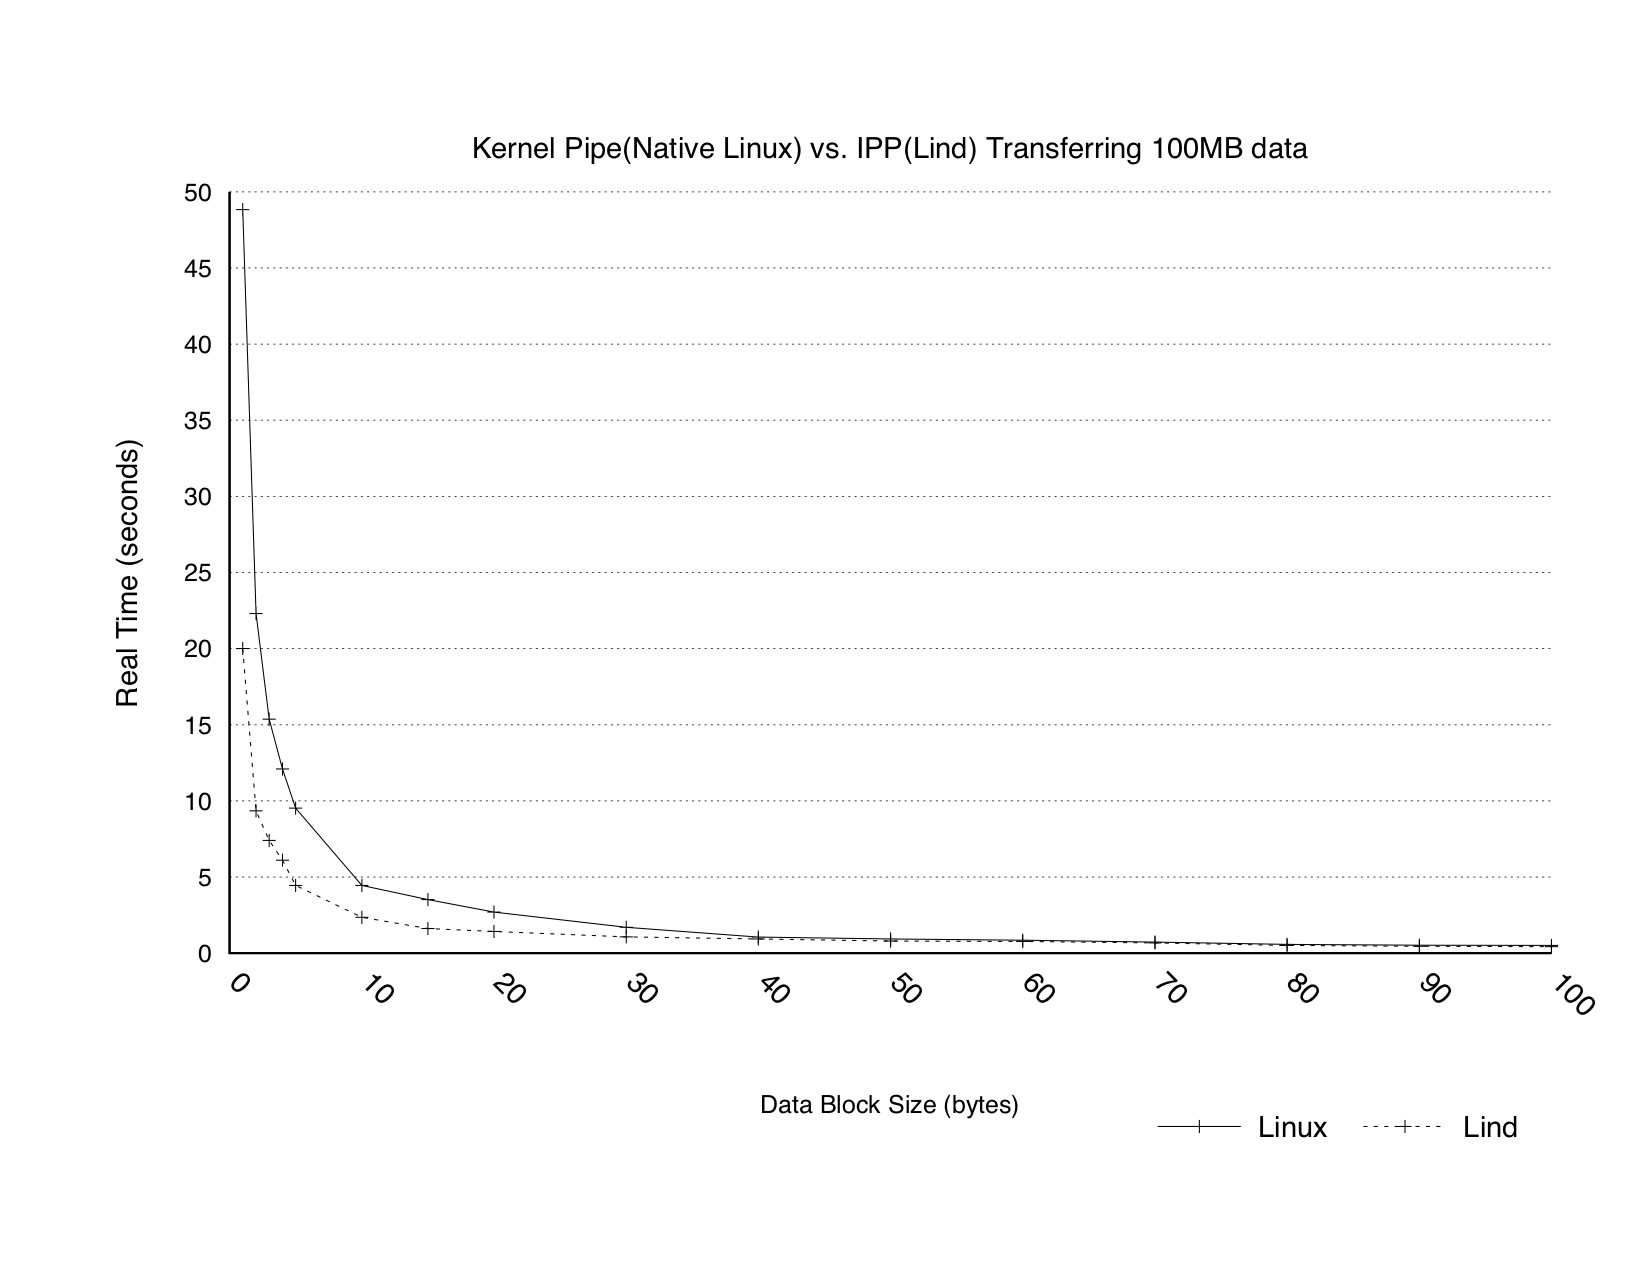
\includegraphics[width=1.0\columnwidth]{diagram/microbenchmarks.png}
\caption{\small Microbenchmarks: Linux vs. IPP.}
\label{fig:microbenchmarks}
\end{figure}

\subsection{Real-World Workloads}
\label{experiments.real-world_workloads}

Next, we conducted experiments on a collection of bash pipeline commands. 
The reasons that we chose bash pipeline commands to run the experiments are: 
first, bash pipeline commands are being widely used by programmers, developers, and researchers 
on Linux and Mac OS. Second, in many cases, bash pipeline commands are easier to use and could be more effective 
than complex programs or tools such as Hadoop. 
We collected and tested a set of real-world bash pipeline commands. Through our experiments, our goal is to demonstrate that 
our \emph{Intra-Process Pipe (IPP)} system provides an attractive solution to speeding up widely used bash pipeline commands 
on real-world workloads. 

We now show the nine real-world bash pipeline commands we tested. Each test was ran under both native Linux and our IPP system. 

\noindent
\textbf{Experiment 1.}

\noindent
\textbf{Setup.}
The following bash pipeline command was from one of the authors' bash history. 
\texttt{grep IOADDR * | sed 's/.*: //' | tr ' ' '\textbackslash n' | sort | uniq -c | sort -n} 
We ran this command on a 1.2GB dataset. 

\noindent
\textbf{Results.}
Results are shown in Figure \ref{fig:results01}. 
We see speedup up to 18\% in our IPP system. 

\begin{figure}
\centering
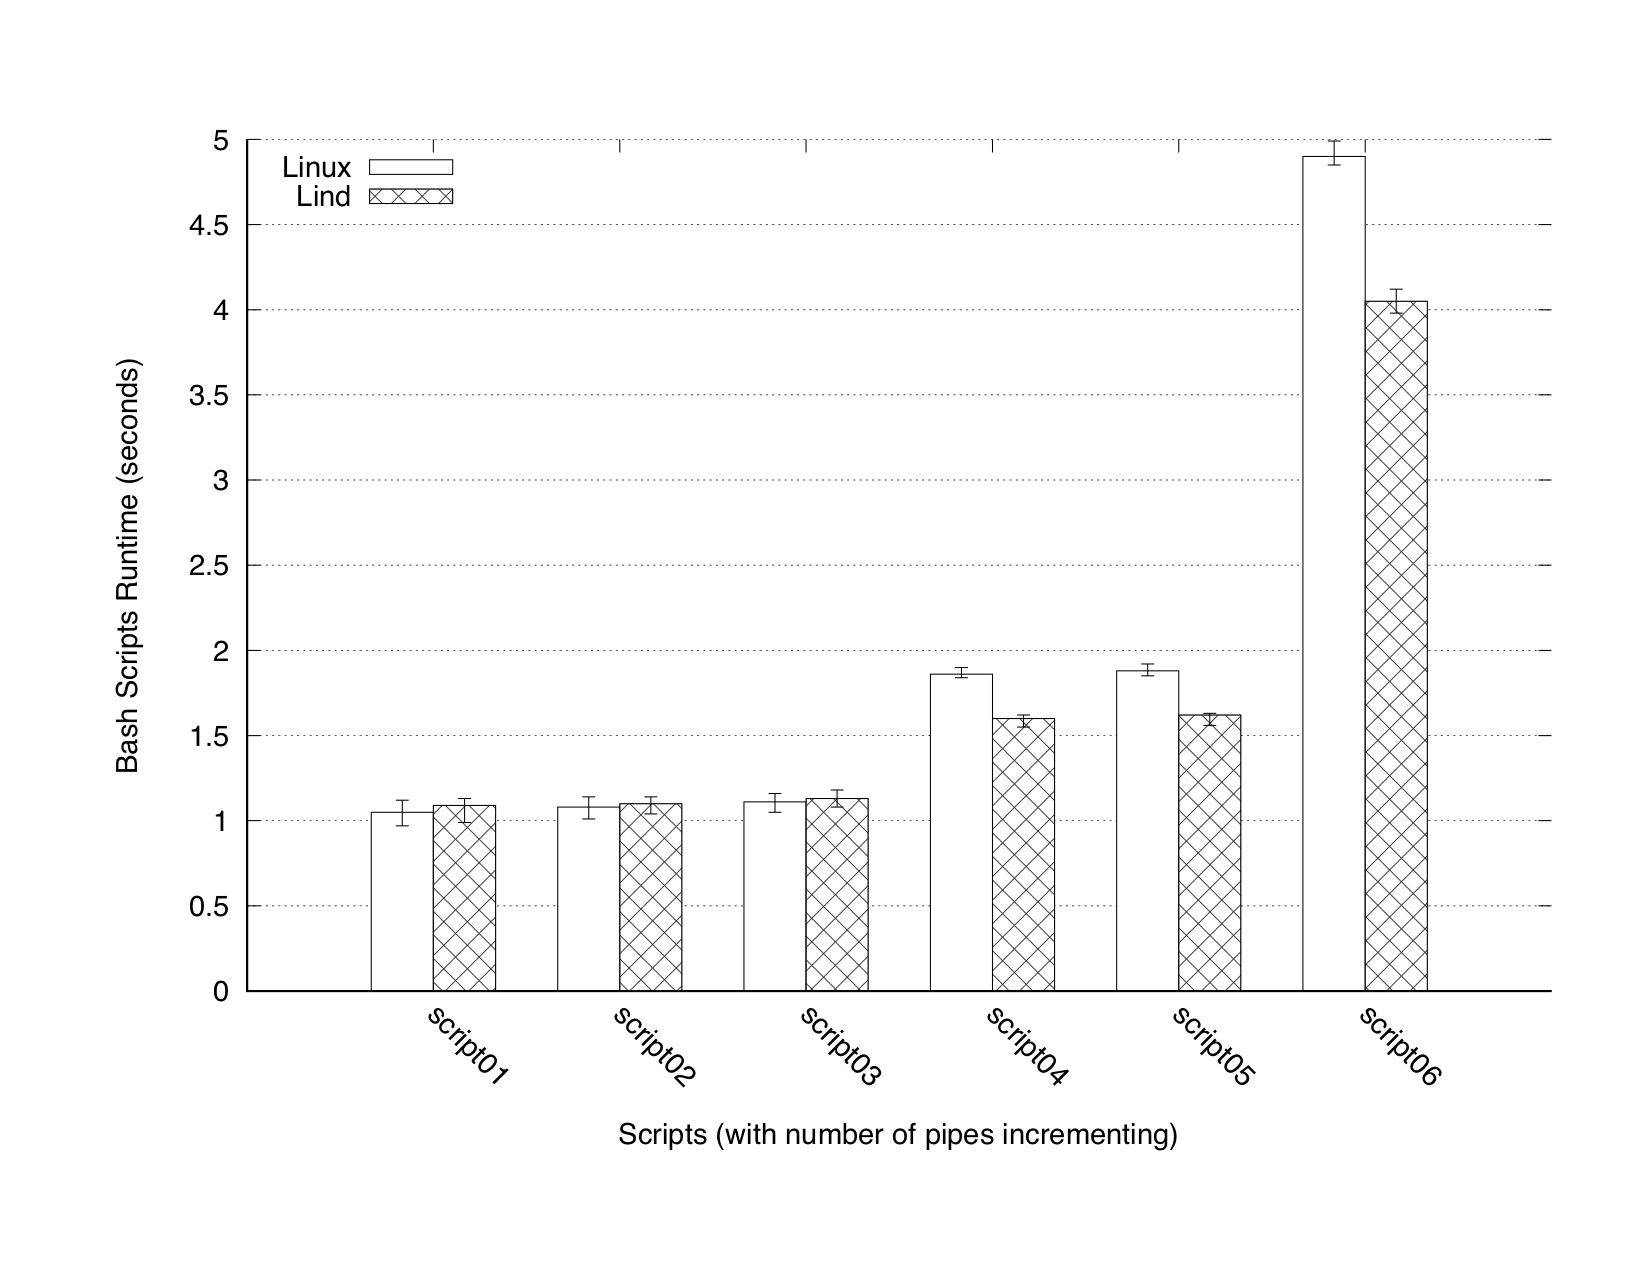
\includegraphics[width=1.0\columnwidth]{diagram/results01.png}
\caption{\small Real-World Workload 1.}
\label{fig:results01}
\end{figure}

\noindent
\textbf{Experiment 2.}

\noindent
\textbf{Setup.}

\texttt{cat ./dataset/pgn/*.pgn | grep "Result" | sort | uniq -c > ./results/results.txt} 


\noindent
\textbf{Results.}
Results are shown in Figure \ref{fig:results02}. 
We see speedup up to 20\% in our IPP system. 

\begin{figure}
\centering
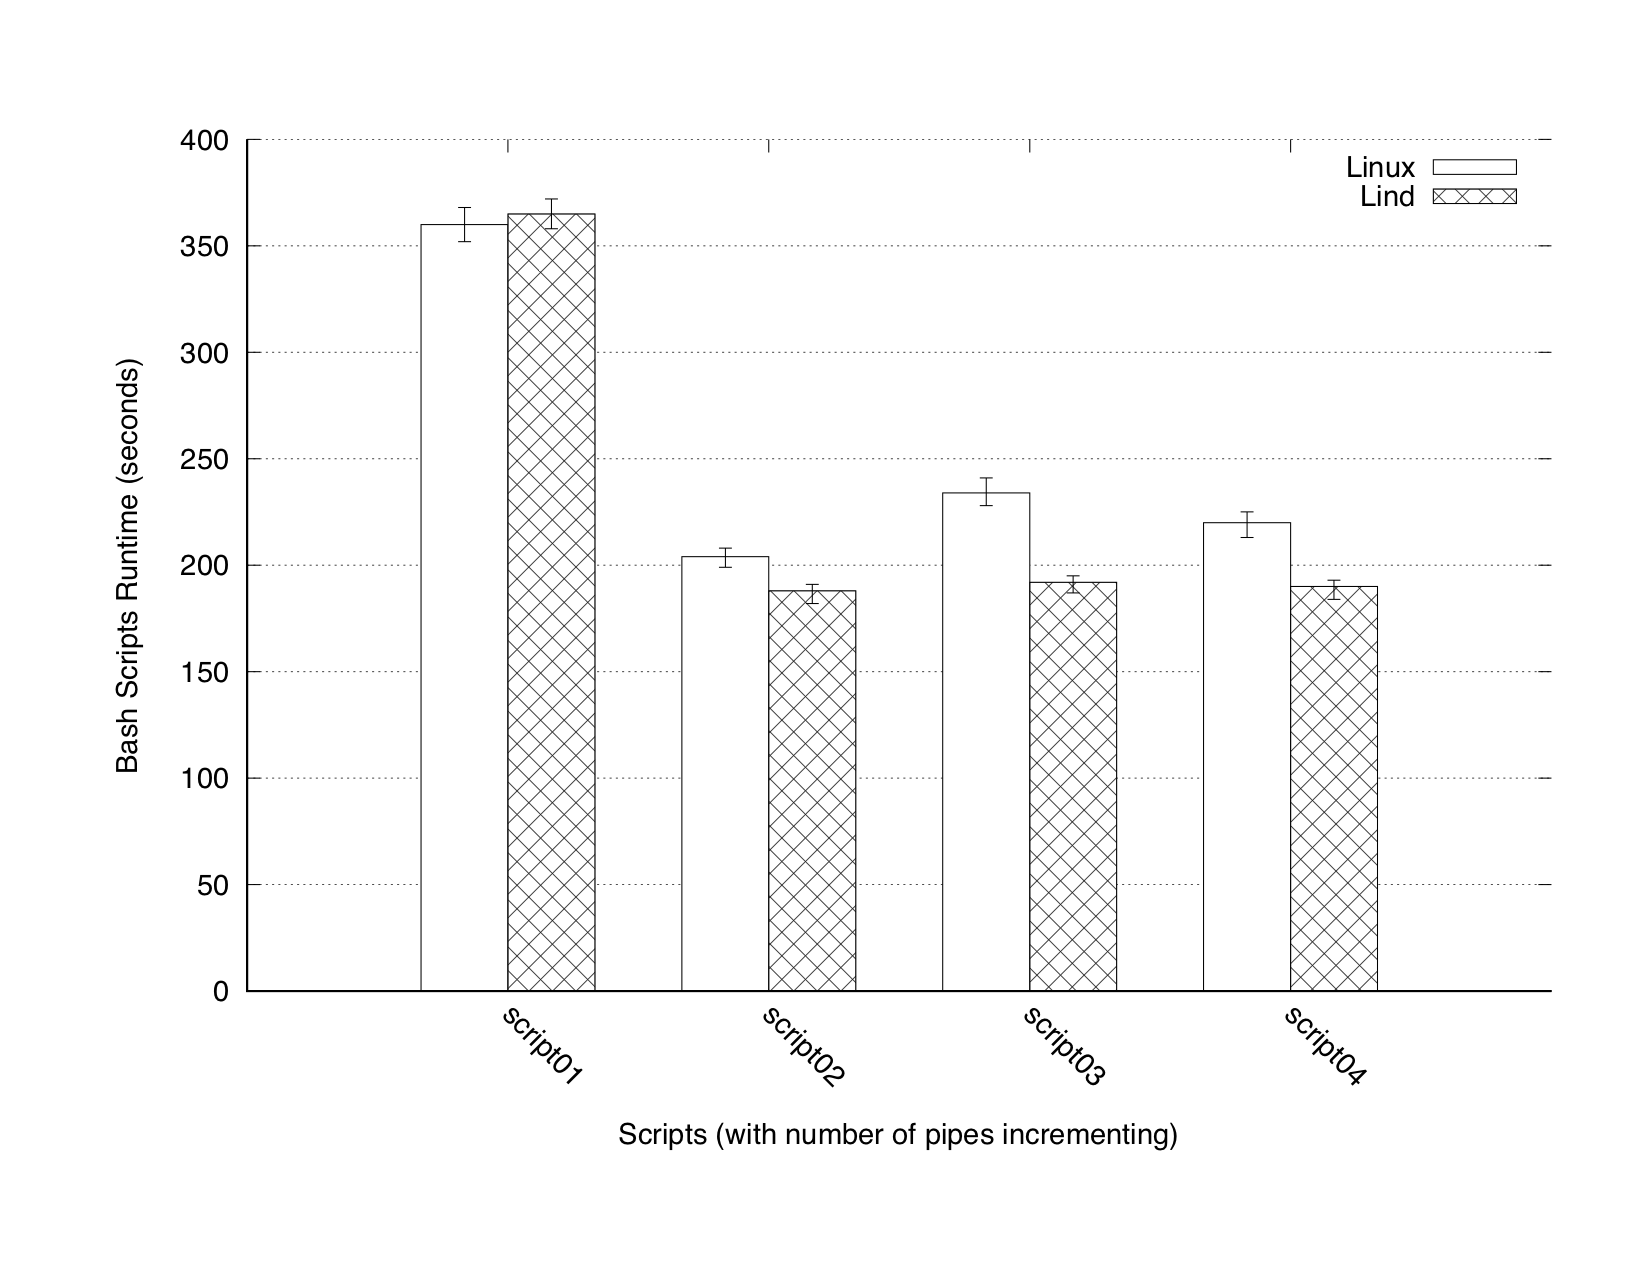
\includegraphics[width=1.0\columnwidth]{diagram/results02.png}
\caption{\small Real-World Workload 2.}
\label{fig:results02}
\end{figure}